% ************
\section{Internet of Things}
\label{c:tec:iot}

La società odierna è sempre più permeata dalla presenza di Internet. La Rete è ormai diventata un bene fondamentale che, se dovesse all'improvviso scomparire, getterebbe nel panico la quasi totalità delle aziende e delle persone. In questo scenario, una tendenza che, da qualche anno a questa parte, sta prendendo piede è che le entità connesse a Internet non siano solo le persone (con i propri smartphone, personal computer ecc.), ma anche gli oggetti: si parla infatti di \textit{Internet of Things} (IoT). Elettrodomestici, sensori, attuatori, dispositivi elettronici di natura eterogenea che, dotati di una scheda di rete, hanno accesso a Internet e possono essere collegati tra loro per formare una rete interconnessa. Esso si riferisce non solo al fatto che gli oggetti possano collegarsi fra di loro, ma anche al fatto che sia esseri umani, sia oggetti fisici, sia ambienti e dati virtuali possono interagire tra di loro nello stesso tempo e spazio.

La forza di questa idea è il grande impatto che avrebbe sui diversi aspetti della vita quotidiana e anche sul comportamento dei potenziali utenti. Se si tratta di un privato, gli effetti dell'introduzione dell'IoT più evidenti sono visibili sia in ambiente lavorativo che in ambiente domestico. La domotica, l'e-health, l'apprendimento potenziato sono solo alcuni esempi delle possibili applicazioni in cui questo nuovo paradigma avrà un ruolo fondamentale nel prossimo futuro. In maniera simile, anche le aziende possono usufruire dell'IoT in campi come l'automazione, la logistica, gestione dei processi, trasporto intelligente di merci e persone. 
Per questi motivi l'Internet of Things può essere considerato, dopo la nascita del World Wide Web negli anni '90 e quella di Internet mobile nel 2000, come la frontiera di Internet potenzialmente più rivoluzionaria.

Le prime applicazioni dell'IoT, nei primissimi anni 2000, furono nel campo manifatturiero con l'impiego della tecnologia RFID (\textit{Radio Frequency IDentification}), attraverso la quale è possibile l'identificazione e la memorizzazione automatica di informazioni legate agli oggetti, consentendo cos\`i di poterli tracciare nel percorso dal centro di distribuzione agli scaffali dei negozi.

Alcuni anni dopo, nel pieno del progresso tecnologico, la diminuzione dell'area occupata dai chip e la riduzione dei consumi energetici, portò allo sviluppo di nuove tecnologie. Un esempio molto importante, che deriva direttamente dai tag RFID, era la tecnologia \textit{Near Field Communication} (NFC), che fornisce connettività wireless a corto raggio con comunicazione bidirezionale.

Un altro importante passo per lo sviluppo dell'IoT fu la creazione delle prime \textit{Wireless Sensor Network} (WSN). Una rete WSN è costituita da un insieme di nodi sensori o \textit{sensor nodes}, cioè componenti in grado di rilevare grandezze fisiche (come la posizione, la temperatura, l'umidità, la luce, o anche il movimento di veicoli, la composizione del terreno, livello di rumore ecc.), di elaborare dati e di comunicare tra loro. I nodi sensore all'interno di una rete hanno la possibilità di collaborare tra loro, dal momento che sono provvisti di un processore on-board; grazie a quest'ultimo, ciascun nodo, invece di inviare dati grezzi ai nodi responsabili della raccolta dei dati, può effettuare delle semplici elaborazioni e trasmettere solo i dati richiesti e già elaborati, cosa che con l'RFID non era possibile. 

Con il passare del tempo, il numero di dispositivi attivi cresceva esponenzialmente di anno in anno, e in più la creazione di reti e protocolli di comunicazione ad hoc per gli oggetti (proprio come nel caso dei sistemi RFID) diventava sempre più superflua in un'epoca in cui Internet, con il suo stack protocollare TCP/IP, si diffondeva a macchia d'olio: l’esigenza che nacque, quindi, era quella di trasformare gli oggetti in semplici nodi di Internet. In altre parole, dovevano possedere un indirizzo IP e usare l'Internet Protocol per comunicare con gli altri oggetti e con gli altri nodi della rete.

Gli oggetti, grazie a questo, diventano \textit{smart objects}, e possono quindi utilizzare i servizi e le applicazioni già esistenti, come il protocollo a livello applicazione HTTP, e diventare effettivi partecipanti non solo di Internet, ma del World Wide Web. 

Un problema che subito si presentava, tuttavia, era la limitata disponibilità di risorse degli \textit{smart objects}, come le capacità computazionali dei processori e i consumi energetici, e quindi dei costi. Uno standard di comunicazione wireless per i livelli 1 e 2 dello stack di comunicazione che presenta consumi relativamente bassi è l'IEEE 802.15.4, conosciuto come \textit{ZigBee}, e venne creato un nuovo protocollo per il livello 3 che si adattava alle caratteristiche di quest'ultimo: è il caso dell'\textit{IPv6 over Low Power Wireless Area Networks} (6LoWPAN).

L'interesse verso questo nuovo standard di comunicazione è cresciuto notevolmente, tanto che sono stati definiti altri protocolli per gli altri livelli dello stack. Un esempio importante è il \textit{Constrained Application Protocol} (CoAP): esso è un protocollo a livello applicazione adatto all’interazione tra dispositivi chiamati, per l'appunto, \textit{constrained}, cioè dalle risorse hardware limitate.

Protocolli come quest'ultimo hanno permesso la formazione dell'insieme di approcci e pattern di programmazione chiamato \textit{Web of Things} (WoT), il quale consente agli oggetti del mondo reale di prendere parte non solo ad Internet, ma al World Wide Web.


%%%%%%%%%%%%%%%%%%%%%
\subsection{Social IoT}
\label{c:tec:siot}
Un'evoluzione che l'IoT ha sub\`ito in tempi molto recenti è l'introduzione del concetto di \textit{social networking} nella sua architettura, formando il cosiddetto \textit{Social Internet of Things}\cite{Atzori2012} (SIoT), che consiste in una rete in cui gli oggetti possono formare delle relazioni e interagire tra loro senza il diretto intervento umano. Questo fenomeno è dovuto ai grandi vantaggi che si verrebbero a creare con questo nuovo paradigma: la navigabilità della rete, che diventa molto più facile, permettendo la ricerca di servizi specifici in modi efficienti; l'introduzione di diversi gradi di affidabilità per regolare il grado di interazione tra oggetti con tipi di relazioni diverse, per avere un certo livello di sicurezza; il riutilizzo dei modelli di studio dei social network per risolvere problemi relativi all'IoT, come la grande estensione della rete di oggetti interconnessi tra loro; la possibilità di stabilire relazioni tra oggetti che usano differenti tecnologie, cosa molto importante per permettere l'interazione tra diverse piattaforme per IoT. In questo scenario, quindi, si può immaginare un mondo popolato da oggetti intelligenti che permeano la vita quotidiana degli esseri umani.

Tuttavia, solo pochi dispositivi IoT hanno le capacità computazionali per poter creare e gestire le relazioni sociali: diventa, quindi, di fondamentale importanza il cloud computing, con il quale è possibile virtualizzare gli oggetti per consentire l'esecuzione, il deployment e il provisioning delle applicazioni. Per implementare il Social IoT, quindi, è necessario impiegare un modello che funga da controparte virtuale degli oggetti fisici, che viene eseguito sui server del cloud, chiamato Social Virtual Object. Le caratteristiche che una piattaforma per il SIoT dovrebbe avere per fornire un buon servizio sono le seguenti:
\begin{itemize}
\item una bassa latenza nel collegamento tra oggetto fisico e corrispettivo digitale;
\item scalabilità, per far fronte al traffico generato dall'enorme numero di dispositivi potenzialmente collegabili;
\item dei social agent autonomi che permettano ai nodi IoT dalle risorse limitate a mantenere e aggiornare le relazioni sociali in maniera consistente;
\item gestione della mobilità, per fornire servizi che si basano sulla posizione dei dispositivi e per consentire la migrazione dei SVO attraverso i server cloud distribuiti geograficamente.
\end{itemize}

Le relazioni che gli oggetti possono stabilire sono le seguenti: la \textit{Ownership Object Relationship} (OOR) si crea tra oggetti appartenenti allo stesso proprietario, la \textit{Co-location Object Relationship} (CLOR) tra dispositivi che si trovano nello stesso luogo, come per esempio gli elettrodomestici di un'abitazione, la \textit{Parental Object Relationship} (POR) tra oggetti che hanno lo stesso modello, produttore e lotto di produzione, la \textit{Co-work Object Relationship} (CWOR) tra oggetti che si incontrano nel luogo di lavoro del proprietario, come ad esempio il computer e la stampante dell'ufficio, infine la \textit{Social Object Relationship} (SOR) tra oggetti che si trovano spesso vicini tra loro, come per esempio gli smartphone delle persone che si trovano ogni giorno sullo stesso autobus per andare al lavoro o a scuola.

Inoltre, possono essere usati due diversi approcci per la costruzione delle reti di oggetti del Social IoT: il primo è quello del Social Web of Things, in cui viene costruito un ecosistema che consente alle persone e agli smart objects di interagire tra di loro all'interno di un unico framework. In questo caso le tecnologie web vengono utilizzate per fornire dei servizi ai nodi della rete. Un secondo approccio, più restrittivo, è rappresentato dal Social Internet of Things in senso stretto, in cui gli oggetti formano legami autonomamente tra loro e sono separati dalle comunità virtuali formate dagli esseri umani, ai quali gli oggetti sono soltanto subordinati.

Sociologicamente la portata di questo cambiamento è molto importante per l'ipotetico spostamento di un paradigma interpretativo che pone al centro proprio l'uomo: macchine al servizio dell'uomo che comunicano con l'uomo.

%%%%%%%%%%%%%%%

\subsection{Piattaforme di virtualizzatione dei nodi IoT}
\label{c:tec:virt}

Le piattaforme di virtualizzazione permettono di ampliare le capacità computazionali dei IoT, dal momento che questi ultimi non sono generalmente dotati di grandi risorse hardware che permettono di immagazzinare la grande quantità di dati generati. Qui di seguito sono illustrate le due piattaforme utilizzate nel sistema, Thingspeak e Festival.

\paragraph{Thingspeak}
\label{c:tec:virt:ts}

Thingspeak è una piattaforma di virtualizzazione open-source realizzata da ioBridge nel 2010. Essa fornisce una serie di applicazioni e di API per poter raccogliere i dati generati dai nodi IoT e poterli processare attraverso il servizio di cloud. Questi vengono poi raccolti in un \textit{channel}, l'elemento primario della piattaforma, dal quale possono essere analizzati, visualizzati, calcolati nuovi dati e possono anche interagire con altri servizi web, come ad esempio i social media e altri dispositivi. Essa fornisce accesso a una grande varietà di dispositivi integrati, come Arduino, Raspberry Pi e BeagleBone Black. 

Thingspeak è open-source, cioè il suo codice sorgente e la lista completa delle API è interamente scaricabile e consultabile dai programmatori di tutto il mondo su GitHub.

Il suo funzionamento si basa su tre principali azioni:

\begin{itemize}
    \item Raccogliere i dati: vengono raccolti tutti quelli provenienti dai vari tipi di sensori (temperatura, pressione, umidità, campo magnetico ecc.), anche sotto forme diverse, come ad esempio valori numerici o segnali elettrici, e vengono inviati nello spazio di cloud riservato al canale.
    \item Analizzare i dati: una volta nel cloud, si possono utilizzare tool di analisi per visualizzare, scoprire relazioni, trend e pattern nei dati. Ciò è possibile grazie alla collaborazione di Thingspeak con \textit{Mathworks}, il quale fornisce gli strumenti di analisi di MATLAB agli utenti della piattaforma senza il bisogno dell’acquisto di una licenza. È possibile convertire, combinare e calcolare nuovi dati, pianificare l’esecuzione di calcoli in momenti ben precisi, usare funzioni built-in per creare grafici, combinare i dati provenienti da più canali analisi più sofisticate. 
    \item Agire sui dati: con l’applicazione \textit{TalkBack}, ad esempio, possono essere innescate delle reazioni al verificarsi di certi eventi, come ad esempio ricevere un tweet quando la temperatura rilevata da un certo sensore supera un determinato valore di gradi Celsius, oppure eseguire operazioni più complesse come azionare un motore. È possibile, quindi, far comunicare i dispositivi collegati alla piattaforma e anche mettere in fila dei comandi da far eseguire a ogni dispositivo. Con questa e con le altre applicazioni presenti nella piattaforma, quindi, è possibile automatizzare e pianificare azioni sia sui dispositivi fisici, sia sul web.
\end{itemize}

\paragraph{Festival}
\label{c:tec:virt:fest}

FESTIVAL è un progetto collaborativo tra Europa e Giappone facente parte di Horizon2020. Esso mira a rendere interoperabili dei testbed eterogenei, appartenenti alle categorie \textit{Open Data} (per esempio dataset), \textit{IoT} (per esempio sensori e attuatori), \textit{IT} (come risorse computazionali) e \textit{Living Labs} (ad esempio persone), per costruire un modello \textit{Experimentation as a Service} (EaaS).

FESTIVAL fornisce anche un insieme di funzionalità per gestire e monitorare gli esperimenti. La piattaforma è stata testata su tre domini di smart city dislocati tra Europa e Giappone: \textit{smart energy}, \textit{smart building} e \textit{smart shopping}.

Per l'implementazione della piattaforma è stato utilizzato il modello EaaS (Experiment as a Service), che permette agli sviluppatori di creare esperimenti replicabili e scalabili e di avere accesso a diversi testbed in maniera trasparente e omogenea. Fornisce inoltre funzionalità di discovery, le quali consentono di trovare le risorse con i requisiti necessari per gli esperimenti e le abilità per analizzare i risultati raccolti durante tutte le fasi degli esperimenti.

L'architettura di FESTIVAL è composta da due livelli: il primo organizza le risorse per categoria, chiamato \textit{“resource-based” federation}, mentre il secondo fornisce accesso a queste ultime (\textit{“experiment-based” federation}), come è possibile osservare in figura \ref{f:tec:festival}.

\begin{figure}[h!t]
\centerline{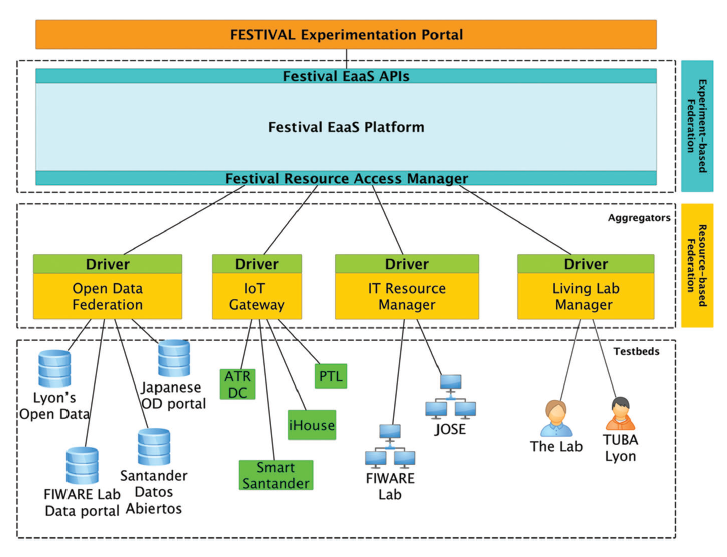
\includegraphics[scale=0.5]{img/festival}}
\caption{Architettura di FESTIVAL}
\label{f:tec:festival}
\end{figure}

Al di sotto di questi livelli è possibile vedere tutti i testbed coinvolti nel progetto, classificati secondo le seguenti tipologie: Open Data, IoT, IT e Living Lab. 

Il livello resource-based fornisce le funzionalità per l'integrazione di ciascun tipo di risorse, utilizzando componenti ad-hoc chiamati Aggregators. Ognuno di questi è indipendente dalla piattaforma, e serve a raggruppare le risorse dello stesso tipo, fornendo un modello dati e una descrizione uniformi. FESTIVAL supporta i seguenti Aggregator:
\begin{itemize}
    \item \textit{Open Data Federation}: esso serve a raggruppare i differenti \textit{Open Data Management Systems} (ODMS), fornendo le funzioni per cercare e per eseguire query sugli open data;
    \item \textit{IoT Gateway}: questo componente è necessario per fornire accesso ai dispositivi IoT, come sensori o smart objects, con i differenti protocolli IoT;
    \item \textit{IT Resource Manager}: esso raggruppa le risorse computazionali, e in particolare è responsabile della gestione di tutti gli aspetti legati alla prenotazione e accesso alle macchine virtuali;
    \item \textit{Living Lab Manager}: questo componente è in grado di raggruppare i living labs, considerando i servizi, metodologie ed esperienza dei loro membri come risorse che possono essere impiegate in un esperimento.  
\end{itemize}

Tutte le funzionalità a livello EaaS sono accessibili da applicazioni esterne attraverso un set di API. FESTIVAL, in particolare, fornisce un'applicazione web progettata per facilitare gli sviluppatori a gestire i propri esperimenti.


% ************
\section{Crittografia: cifratura asimmetrica}
\label{c:tec:cifratura}

La cifratura a chiave simmetrica è un meccanismo secondo il quale la stessa chiave viene utilizzata sia per cifrare che per decifrare; è molto intuitiva, dal momento che è un concetto molto vicino alla nostra quotidianità, l'aprire e chiudere una porta con la stessa chiave.
Questa caratteristica richiede meccanismi sofisticati per distribuire la chiave alle parti che comunicano in maniera sicura, visto che una volta scoperta la chiave di cifratura l'intera comunicazione è compromessa.

La cifratura asimmetrica, invece, introduce il concetto di avere non una, ma due chiavi: una per cifrare, l'altra per decifrare\cite{Cgi2004}. Questo meccanismo presenta molti vantaggi rispetto alla cifratura a chiave simmetrica:
\begin{itemize}
    \item distribuzione delle chiavi semplificata;
    \item \textit{Digital Signature};
    \item cifratura a lungo termine.
\end{itemize}

Ad ogni modo, la cifratura \textit{symmetric key} rimane ancora il principale metodo di implementazione delle \textit{Public-key Infrastructure} (PKI).

La componente principale della cifratura asimmetrica è la coppia di chiavi: una \textit{public key} e una \textit{private key}. La prima viene resa pubblica e quindi distribuita liberamente, mentra la seconda deve essere mantenuta segreta e mai distribuita. 

Dato un paio di chiavi, i dati che vengono cifrati con la public key possono essere decifrati solo con la private key, mentre i dati cifrati con la chiave privata vengono decifrati con la chiave pubblica. Questi meccanismi vengono utilizzati per realizzare, rispettivamente:
\begin{enumerate}
    \item \textit{Confidentiality} (solo il possessore della private key può leggere i dati cifrati con la chiave pubblica corrispondente). La cifratura è un meccanismo per cui un messaggio viene trasformato in modo tale da poter essere letto da mittente e destinatario. Per esempio, si supponga che Alice voglia inviare un messaggio a Bob. Per farlo, ha bisogno la chiave pubblica di Bob; visto che lui può mandarla attraverso la rete senza problemi, Alice cifra il messaggio utilizzando questa public key e lo manda a Bob. Egli riceve il messaggio e, utilizzando la sua chiave privata, è in grado di decifrarlo.
    \item \textit{Integrity} e \textit{authentication} attraverso la firma digitale: è un meccanismo per cui un messaggio viene autenticato, per esempio provando che proviene effettivamente da un certo mittente, proprio come una firma in un documento cartaceo. Per esempio, supponendo che Alice voglia apporre una firma digitale a un messaggio diretto a Bob. Per fare ciò, utilizza la propria private key per cifrare il messaggio e poi invia il messaggio cifrato con in più la propria chiave pubblica. Dal momento che la sola chiave che può decrittare il messaggio è la chiave pubblica di Alice, una decifratura che va a buon fine rappresenta una \textit{Digital Signature Verification}, cioè è la prova inconfutabile che il messaggio è stato cifrato con la chiave privata di Alice.
\end{enumerate}

% ************

\section{Blockchain e Bitcoin}
\label{c:tec:blockchain}

Una blockchain è un database distribuito che contiene record di un \textit{public ledger} (libro mastro) di tutte le transazioni o eventi digitali che sono stati eseguiti e condivisi tra le parti che vi partecipano. Ogni transazione nel public ledger viene verificata dal \textit{consenso} della maggioranza dei partecipanti nel sistema. E, una volta dentro, l'informazione non può più essere cancellata. La blockchain contiene un record verificabile di ogni singola transazione che sia stata mai fatta.

Per usare una metafora, è più facile rubare un biscotto da una scatola tenuta in un luogo nascosto rispetto a rubarlo da una scatola che si trova in piena vista in un supermercato davanti a migliaia di persone.

\textit{Bitcoin} è l'esempio di utilizzo della tecnologia della blockchain più famoso, ma anche più controverso, dato che rende possibili transazioni multimiliardarie nel mercato globale che sono totalmente anonime e fuori da ogni controllo delle autorità \cite{Nakamoto2008} \cite{BitcoinProject2014}. 

In ogni caso, la Blockchain di per sè non è per niente controversa, ed è stata impiegata in applicazioni sia finanziarie che non finanziarie con risultati impeccabili. Il modello di consenso distribuito della blockchain è stato addirittura incluso tra le invenzioni più rivoluzionarie dall'invenzione di Internet stesso da Marc Andreessen, uno dei più importanti imprenditori della Silicon Valley \cite{Crosby2016}.

L'economia digitale odierna si affida a delle \textit{trusted authority} per praticamente qualsiasi cosa: tutte le nostre transazioni online si basano sul fatto che esiste qualcuno che ci dice cosa è vero, ad esempio come un provider di un servizio email che ci dice che la nostra email è stata inviata; o come un social network che ci oppure come una banca che ci conferma che i nostri soldi sono stati inviati in maniera sicura ai nostri cari in un'altra nazione. In sostanza, viviamo precariamente la nostra vita digitale perch\'e contiamo su queste terze parti per la sicurezza e privacy dei nostri beni digitali. Il problema principale, però, è che queste possono essere hackerate e compromesse in qualche modo.

È proprio qui che la blockchain viene in aiuto: essa ha il potenziale per rivoluzionare il mondo digitale consentendo di raggiungimento di un consenso distribuito in cui qualsiasi transazione che coinvolga beni digitali può essere verificata in qualsiasi momento, senza compromettere la privacy dei beni e delle parti in questione. 

\subsection{Funzionamento}
\label{c:tec:blockchain:funzionamento}

Per spiegare i concetti alla base dalla blockchain è doveroso portare in esempio il funzionamento del sistema dei Bitcoin, dato che sono entrambi interconnessi. Ciò non toglie che la blockchain sia applicabile in qualsiasi altro ambito e bene digitale che viene scambiato online.

Il commercio su Internet è esclusivamente legato al fatto che le istituzioni finanziarie fungono da terza parte, la quale processa e media qualsiasi transazione elettronica. Il ruolo di una terza parte \textit{trusted} è quello di validare e salvaguardare le transazioni per evitare che avvengano frodi. Tutto ciò comporta alti costi.

Bitcoin, in un contesto in cui due parti vogliano eseguire una transazione su Internet, utilizza una prova crittografica invece della fiducia nella terza parte. Ogni transazione viene protetta da una firma digitale, cioè viene firmata con la \textit{private key} del mittente e poi inviata alla \textit{public key} del destinatario. Per poter spendere quei soldi, il proprietario della valuta deve dimostrare la proprietà della private key: per fare ciò, l'entità che riceve il denaro verifica la firma digitale della transazione utilizzando la public key del mittente.

Ogni transazione viene inviata in broadcast a tutti i nodi della rete Bitcoin e, dopo essere stata provata la sua validità, viene registrata in un \textit{public ledger} (libro mastro pubblico). Il nodo che effettua questa verifica deve assicurarsi che siano rispettati i seguenti requisiti:
\begin{enumerate}
    \item il mittente è il proprietario della firma digitale della transazione;
    \item il mittente possiede sufficiente criptovaluta nel suo account: bisogna cercare nel public ledger ogni transazione compiuta verso la sorgente della transazione (nello specifico la sua public key) per confermare che essa abbia credito sufficiente.
\end{enumerate}

Tuttavia, si presenta il problema del mantenimento dell'ordine delle transazioni che vengono diffuse nella rete peer-to-peer Bitcoin: non vi è, infatti, alcuna certezza che le transazioni siano disposte nell'ordine in cui vengono generate, considerato che esse vengono passate di nodo in nodo attraverso la rete, ed è quindi necessario un sistema per evitare qualsiasi attacco di \textit{double-spending}\footnote{\url{https://en.bitcoin.it/wiki/Irreversible_Transactions}}: come il nome stesso definisce, si ha quando viene speso un certo ammontare di valuta più di una volta. Nei sistemi tradizionali il problema non sussiste, visto che la terza parte fa da garante delle transazioni. Nella blockchain, però, non essendo essa un sistema centralizzato, non si ha nessuna garanzia sul fatto che una certa quantità di denaro non sia già stata spesa da qualche altra parte.

Questo comporta il bisogno di sviluppare un meccanismo per il quale l'intera rete Bitcoin può concordare sull'ordine delle transazioni, un problema che da sempre ha caratterizzato i sistemi distribuiti tradizionali. Esistono in letteratura, infatti, diversi algoritmi per il raggiungimento del consenso, come ad esempio Paxos\cite{Lamport2001}.

Il problema del consenso, però, non è ancora risolto: come può la rete decidere quale blocco dovrebbe essere aggiunto nella Blockchain dal momento che qualunque nodo è in grado di raccogliere transazioni non confermate, creare un blocco e diffonderlo nella rete? Più blocchi, inoltre, possono venire creati da nodi differenti nello stesso momento e, trovandoci in una rete decentralizzata, non si può risalire all'effettivo ordine di creazione dei blocchi stessi.

La soluzione adottata nella blockchain della rete Bitcoin è geniale nella sua semplicità: ogni blocco viene ammesso nella blockchain solo se risolve un \textit{rompicapo matematico}. Il nodo che per primo riesce a trovarne la soluzione ha il permesso di aggiungere il blocco appena \textit{estratto} nella Blockchain. 
Questo meccanismo è conosciuto come \textit{Proof of Work} (PoW).

\begin{figure}[h!t]
\centerline{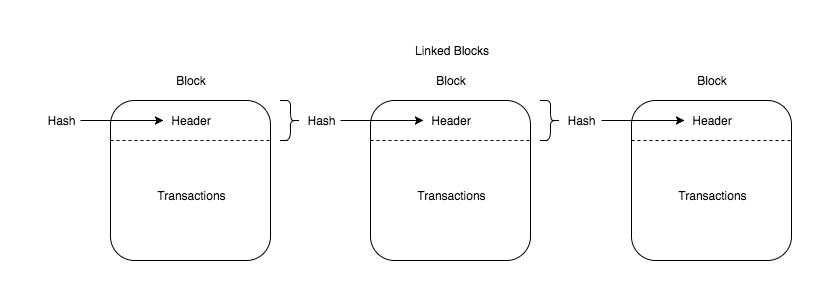
\includegraphics[scale=0.5]{img/blockchain}}
\caption{Schema semplificato di una blockchain}
\label{f:grids:arch}
\end{figure}

\subsection{Proof of Work}
\label{c:tec:bitcoin:pow}
L'algoritmo PoW consiste nel cercare un valore il cui hash (calcolato per esempio con SHA-256), quando viene calcolato, comincia con un certo numero di bit a zero. Il lavoro medio richiesto per trovare questa soluzione cresce in modo esponenziale al numero di bit nulli richiesti nell'hash e può essere verificato in modo estremamente semplice, ossia facendo l'hash del blocco.
Nel caso della rete Bitcoin, ogni blocco contiene un \textit{nonce} che viene incrementato finché il valore dell'hash non è quello desiderato. Questo processo richiede un certo \textit{lavoro} da parte della CPU appartenente al nodo "vincitore", e il blocco non può essere cambiato senza fare nuovamente il lavoro. In più, quando vengono accodati nuovi blocchi, il lavoro per modificarlo include anche il lavoro per modificare tutti gli altri blocchi che lo seguono. La caratteristica chiave che rende la blockchain immutabile è il fatto che, al variare anche solo di un singolo bit di un blocco, il suo hash cambia completamente, e quindi non contiene più il numero di bit più significativi a zero richiesti dal PoW. 
L'algoritmo risolve anche la questione di determinare la rappresentazione dei voti: se si basasse sul principio one-IP-address-one-vote, potrebbe essere facilmente sovvertito da qualsiasi attaccante che allocasse tanti indirizzi IP - questo attacco è conosciuto in letteratura come \textit{Sibyl Attack}, spiegato più avanti nel paragrafo \ref{c:integr:lib:bitcoinj}. La Blockchain si basa, invece, sul principio one-CPU-one-vote: la decisione adottata dalla maggioranza è rappresentata dalla catena più lunga, alla quale è stato investito il maggior sforzo computazionale. Se la maggioranza della potenza delle CPU della rete è controllata da nodi \textit{trusted}, la catena "onesta" sarebbe quella a crescere più velocemente e a superare tutte le altre; per modificare la blockchain, inoltre, un attaccante dovrebbe rieseguire il PoW del blocco che vuole modificare e di tutti quelli che lo seguono, e quindi dovrebbe equagliare e sorpassare il lavoro di tutti i nodi \textit{trusted}, cosa impossibile da fare per una minoranza.

Per compensare l'incremento della velocità dell'hardware, la difficoltà del PoW viene determinata da una media mobile del numero di blocchi creati all'ora: se vengono generati troppo velocemente, la difficoltà aumenta, in modo tale da mantenere la velocità a un blocco ogni circa 10 minuti. 
C'è una probabilità molto bassa che vengano generati più blocchi contemporaneamente, ma se dovesse accadere la blockchain, invece di "dividersi" come ci si aspetterebbe, si stabilizza velocemente.

I nodi che donano la loro capacità computazionale per risolvere il \textit{puzzle} e di fatto costruire la blockchain vengono chiamati \textit{miners}, e vengono premiati ogni volta che risolvono un blocco.


\subsection{Altri algoritmi di consenso: Proof of Stake}
\label{c:tec:bitcoin:pow}

Sono stati trattati in letteratura, oltre al PoW, altri algoritmi di consenso distribuito adatti all'utilizzo nella blockchain: uno di questi è il \textit{Proof of stake} (PoS)\cite{Li2005}. Nelle criptovalute PoS-based, come PeerCoin, il creatore del blocco successivo viene scelto in base a varie combinazioni tra selezione random, ricchezza o età (da qui la parola \textit{stake}, partecipazione).

Ci sono diverse tecniche di selezione del blocco, tra cui:

\begin{itemize}
    \item \textit{Randomized block selection}: Nxt e BlackCoin utilizzano la randomizzazione per designare il miner successivo, attraverso l'uso di una formula che va a vedere il valore di hash più piccolo insieme alla misura dello stake. Dal momento che questi ultimi sono pubblici, ogni nodo può predirre con ragionevole precisione quale nodo vincerà il diritto di estrarre un blocco.
    \item \textit{Coin age-based selection}: è il caso di Peercoin, il cui sistema combina la randomizzazione con il concetto di \textit{coin age}, un numero derivato dal prodotto del numero di monete per il numero di giorni in cui il denaro è stato mantenuto. Ciò vuol dire che insiemi di monete grandi e "vecchi" possono competere per generare il blocco successivo, però l'età viene azzerata non appena viene firmato un blocco e quindi il proprietario di quelle monete deve ricominciare da capo; inoltre, la probabilità di trovare il blocco successivo raggiunge il massimo valore dopo 90 giorni, in modo da evitare che si formino insiemi troppo "vecchi" di stake che dominerebbero la blockchain. Questo processo rende sicura la rete e produce gradualmente nuove cripto-monete col passare del tempo, senza consumare eccessive quantità di potenza computazionale. 
    \item \textit{Delegated Proof of stake} (DPoS): i sistemi che utilizzano questa modalità utilizzano un numero limitato di nodi per proporre e validare i blocchi. Ciò serve a mantenere i tempi di processamento delle transazioni bassi. EOS, ad esempio, utilizza soltanto 21 miners, la cui reputazione può aumentare o diminuire, consentendo ad altri nodi di sostituirli. 
    \item \textit{Randomized Proof-of-Stake} (RPoS): simile al DPoS, ma viene selezionata una "commissione" piuttosto che un nodo singolo. Ogni nodo viene scelto casualmente utilizzando un \textit{beacon} verificabile per proporre il blocco corrente di transazioni, e poi quest'ultimo viene verificato attraverso quel comitato di nodi.
\end{itemize}
